\documentclass{article}
\usepackage[utf8]{inputenc}
\usepackage[margin=0.8in]{geometry}
% !TeX spellcheck = en_US 
%programming code package
\usepackage{listings}
\usepackage{color}

 \usepackage{float}
\usepackage{graphicx}
\graphicspath{ {./images/} }

\definecolor{dkgreen}{rgb}{0,0.5,0}
\definecolor{gray}{rgb}{0.6,0.6,0}
\definecolor{mauve}{rgb}{0.58,0,0.82}
\setcounter{secnumdepth}{3}
\lstset{frame=tb,
  language=Python,
  aboveskip=5mm,
  belowskip=5mm,
  showstringspaces=false,
  columns=flexible,
  basicstyle={\small\ttfamily},
  numbers=none,
  numberstyle=\color{red},
  keywordstyle=\color{blue},
  commentstyle=\color{dkgreen},
  stringstyle=\color{mauve},
  breaklines=false,
  breakatwhitespace=true,
  tabsize=4,
  otherkeywords={self},             % Add keywords here
  keywordstyle=\color{blue},
  emph={Class,__init__},          % Custom highlighting
 emphstyle=\color{red},    % Custom highlighting style
  %emph={1,2,3,4,5,6,7,8,9},          % Custom highlighting
  %emphstyle=\color{red},    % Custom highlighting style
  %stringstyle=\color{green},
}

%\title{MTSubreflector Communication Class}

\newcommand{\HRule}[1]{\rule{\linewidth}{#1}}

\title{ \normalsize \textsc{Effelsberg 100m Radio Telescope}
		\\ [2.0cm]
		\HRule{0.5pt} \\
		\LARGE \textbf{\uppercase{Subreflector Program \\Programmers Manual}}
		\HRule{2pt} \\ [0.5cm]
		}
		
		
\author{
		Created by: Ivan Sharankov \\ 
		Contact: ivansharankov3@gmail.com \\
		}
%\email{ivansharankov3@gmail.com}
\date{\today}

%\title{ \normalsize \textsc{Effelsberg 100m Radio Telescope}
%		\\ [2.0cm]
%		\HRule{0.5pt} \\
%		\LARGE \textbf{\uppercase{Subreflector Program \\Users Manual}}
%		\HRule{2pt} \\ [0.5cm]
%		\normalsize \today \vspace*{5\baselineskip}}


\begin{document}



\maketitle
\newpage

\tableofcontents
\newpage




\section{Introduction}

The goal of this manual is to give an in-depth explanation regarding the structure of the new MT Subreflector communication program that I have developed over my four months working as an intern at the Effelsberg 100m radio observatory.  Overall, the documentation  is kept in a formal tone; but since this was a personal project (and this document will mainly be kept internally), some sections may use an an informal tone regarding discussions of what I did, why I did it that way, and what my thought process was. 

\vspace{10pt}

Mane of the names in this module are currently up for change. If you have any advice for a clearer name upon reading a section, I would be happy to hear it. Specifically a better naming scheme for the modules, as subreflector\_client.py, subreflector\_program.py, and mock\_subreflector are a jumble to repeat.


\newpage
\section{Structure Overview}

The main structure of this project can be currently explained between five core modules, and how they communicate and interact with each other. Other modules do exist, like config.py or process\_message.py, but these are mainly helper modules with added functionality that is separated to be used in multiple locations more freely, as a means to clear up clutter in the main modules. The main structure can be seen in the figure below:

 \vspace{10pt}

 \begin{figure}[H]
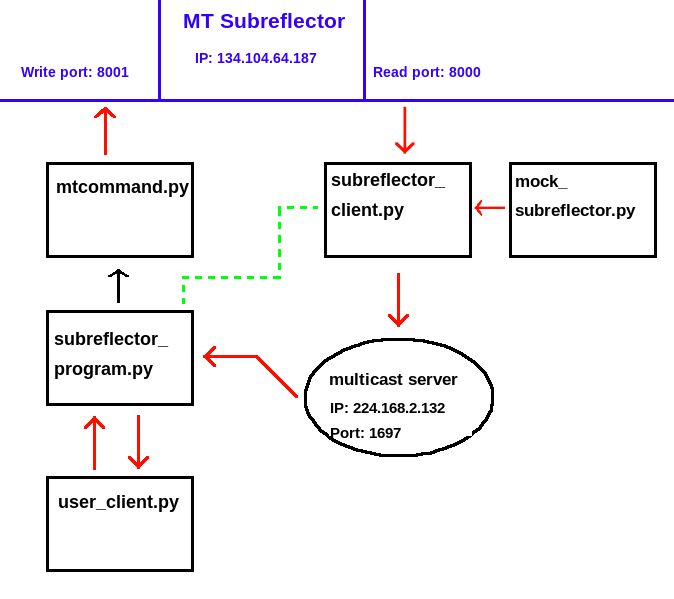
\includegraphics[width=16cm, height=16cm]{program_diagram}
\centering
\end{figure}


 \vspace{10pt}

Tips for understanding the above diagram. Boxes represent individual modules in the program. Each box is a specific module, with its name given in the box. The top shows the subreflector, and separates the read and write ports on the subreflector.  The arrows show which way data/information is passed between modules. Red arrows represent sockets between two modules, while the black arrow between subreflector\_program.py and mtcommand.py represents the method calls being done from subreflector\_program.py. The green dotted line between subreflector\_program.py and subreflector\_client.py represents the fact that subreflector\_client.py is started up in a thread in subreflector\_program.py, such that when subreflector\_program.py is ran, subreflector\_client.py is also setup. The multicast server is represented as a circle, since it is not actually anywhere physical on the system like the modules are.


 \vspace{10pt}
% Basic explination of user_client.py
A more thorough explanation of each module is given in the next section, where every module will individually be explained in depth, and how they work. Starting from the bottom, we have the user\_client.py module. This is a very simple module that asks the user for a IP address and port. Once parsed, it calls an instance of subreflector\_program.py  and if the users asks, an instance of mock\_subreflector.py as well. Both these are then run in the background. This user\_client.py then simply asks the user an input message to send to the program. When received (whatever the message may be), the message is sent to the subreflector\_program.py through the socket (usually at the address/port combo (`', ***REMOVED***)).

 \vspace{10pt}

% Basic explanation of subreflector_program.py
From here, subreflector\_program.py receives the message in a special socketserver class, MyUDPHandler, a threaded UDP class. This class receives any message on the client port (`', ***REMOVED***), and then calls  a method in the class CommandParser, passing on the user message along. CommandParser receives this message, parses it for contents, and does the respective task (if any) given by the user. Most of the correct inputs by the user are commands to the subreflector (specified and described in the users manual). If the user message is found to contain a command for the subreflector, the corresponding method in the mtcommand.py class MTCommand, is called (with any parameters if necessary).  All of the MTCommand methods called will automatically structure the command, package it to represent a C struct (necessary as the current subreflector is running on C, and only recognizes C type structures),  and send the message to the Subreflector via a socket. If the user input is not a subreflector command, the user input usually calls a separate class for accessing the multicast data from the subreflector, explained later. From here, CommandParser returns to MyUDPHandler various messages gain while parsing the message, and these messages are then sent back to the user for confirmation as to how their input message was received. 

 \vspace{10pt}
 
 % Basic explanation of Subreflector_client.py 
Next, the subreflector\_client.py. This module is instantiated in its own thread  during the setup of subreflector\_program.py.  The job of subreflector\_client.py is fairly simple; it  processes all the data returned from the subreflector on port ***REMOVED*** (the read port), and packages that data to a multicast server. This multicast server can then be accessed by any client to read the subreflector data. subreflector\_client.py does use the module process\_message.py for some of its analysis of the incoming data (mainly to structure, organize, and make the data human readable), but this is explained later. If mock\_subreflector.py is called and is running (initiated upon user request), then subreflector\_client.py receives data from the mock subreflector rather than from the real one. This is useful while testing or when access to the real subreflector is not possible. 

\vspace{10pt}

% Multicast functionality in subreflector_program explained
Lastly, we arrive back at the subreflector\_program.py again. This module also listens to the data received on the multicast server via a class called MulticastReceiver. This data can be used to make sure the subreflector status matches saftey requirements  (i.e hexapod is active before a move hexapod command is given), as well as receiving current elevation/motor statuses upon user request. This information is the passed back to the MyUDPHandler, which then goes back to the user at the user\_client.py module.

\vspace{10pt}

% Conclusion 
This wraps up the very basic overview of how the different modules work, their purpose, and most importantly, how the modules communicate with each other. A  more in-depth explanation of each module is given in the next section. 




\newpage
\section{In-depth module explanations}

This section will aim to give a thorough  explanation of the functionality of each module in this system, with explanations of each class, function, and even most individual methods.  Just as the goal of section 2 was to have the reader understand the basic overview of the whole program, and how the modules connect/pass information to each other, this section aims to do the same on a module level. After reading any subsection below, the reader should hopefully be able to go as far as to jump into the source code and start editing and modifying the module with a clear understanding of how the module functions (but please update this if you do!)

 


% % % % % USER CLIENT MODULE % % % % %
\subsection{user\_client.py}
 With the current setup, this is the only module the user should ever initiate. Everything else is ran and started in their own threads through the input given by the user during the start-up process of user\-client.py. 
 
 \subsubsection*{main()}
 
 Once run, this module first asks the user for a IP/port combo. The port is checked to be between ***REMOVED*** and 65535, the IP address has no such checking. Currently, the functionality of this program expects the program to be run locally (i.e. on the same machine that user\_client.py is ran), but this can easily be changed in this module when/if the program replaces the current setup and is run on a server. If that is the case, then some edits to this module would make accessing this program remotely (like you do with udp-telnet) possible. This IP address and port combo will try to connect to an instance of the subreflector\_program.py module. As both are local to the same machine, ` ` or `0' both will try to bind to a local socket. `' or `0' should be imputed if the running instance of the program is expected to be locally on that machine. If subreflector\_program.py is on a server somewhere (like with udp-telnet), a different address would be used. The port for communication with the subreflector\_program.py is currently ***REMOVED***. The below lines check if the address given by the user are for the local system. If this is true, ask\_user\_between\_test\_and\_real\_server() is called. 

    \begin{lstlisting}
               if address in ['', '***REMOVED***']:
                    ask_user_between_test_and_real_server()
    \end{lstlisting}

\subsubsection*{ask\_user\_between\_test\_and\_real\_server()}

This helper function asks the user to return `mock' or `test' if an instance of mock\_subreflector.py should be ran, or `real' if one should not be run as the user wishes to connect to the real subreflector. In either scenario, subreflector\_start\_server.main() is also called, which starts up subreflector\_program.py so that the user messages from user\_client.py actually have a destination to be received at. This logical reasoning can be changed depending how you would like the implementation to work. Once connected, with all the respective modules called to run as well, user\_client.py then runs in an infinite loops asking the user for any inputs, of which all go to the subreflector\_program.py module to be parsed. If a quit() function would be desired for cleanup, here is a useful place to implement one. 

\vspace{10pt}

This module also uses the recv\_msg() helper function, located in process\_message.py and described in that subsection.


\newpage
% % % % % SUBREFLECTOR_PROGRAM MODULE % % % % %
\subsection{subreflector\_program.py}

\subsubsection*{main}

The main function in this module sets up the logging info, and then tries to start the two threads. The first thread is started by instantiating  the ClientModule class, and then calling the start\_sr\_client() method. The second thread set up a non-daemon thread to initiate the ThreadingUDPServer in the background. This is the code that connects to the user to read the command message and parse it.


\subsubsection{ThreadingUDPServer}

This class is part of a set of built-in classes provided with socketserver. It adds threading functionality to a server and does most of the overhead for you. Only special thing to note here which deviates from the standard socketserver implementation of a ThreadedUDPServer is the instance variable self.command\_parser, which instantiates a CommandParser so MyUDPHandler can access it.


\subsubsection{ClientModule}
The ThreadedUDPServer class is started in a basic thread with threading.Thread(target=....). This approach is not used with the subreflector\_client.py  module as ClientModule needs to be accessed by the user to reset the connection. For this reason, ClientModule is a class whose main functionality is to start a threaded instance of the SubreflectorClient class in subreflector\_client.py, but also has extra methods to initiate a shutdown and connection reset of SubreflectorClient if necessary.

TODO add small descriptions for modules.  %%%%%%%%%%

\subsubsection{MyUDPHandler}

MyUDPHandler uses the socketservers' BaseRequestHandler to detect incoming messages on the given address. The handle method is ran every time a message is received through the user\_client.py socket. All this handle method does is decode the message and pass it through to the CommandParser class. It then receives all the messages collected by the CommandParser class and relays them back sequentially to the user in a for loop.

\subsubsection{CommandParser}

TODO%%%%%%%%%%%%%


\subsubsection{MulticastReceiver}

TODO%%%%%%%%%%%%%%%%

%\subsubsection*{check\_if\_command\_sent\_successfully() }



% % % % % MTCOMMAND MODULE % % % % %
\newpage
\subsection{mtcommand.py}

This is the only module that maintains a direct link with the write port of the subreflector. Because of this, mtcommand.py has the core functionality required for communicating with the subreflector. Excluding  the overhead structure classes, the encapsulate command, and other minor methods, most of the MTCommand class (the sole class in the whole module) is populated with methods that directly follow the remote control interface (EFB-SPE-4710-03)  documentation of how to structure a command.

\vspace{10pt}
The self.msg instance variable is used to pass messages onto the user through the CommandParser class, in the scenario an error is to arise while packaging the message. When CommandParser calls any method in MTCommand, it also checks the MTCommand instance variable self.msg to see if it is ``sent successfully'', a message only returned if the command is successfully structured, packaged, and sent to the subreflector. If for any reason MTCommand fails to structure the command, it will of course be logged, but the message will be something other than ``sent successfully'', which is then conveyed back to the user using the check\_if\_command\_sent\_successfully() method in CommandParser.  The reasoning for this structuring is explained a bit more in recv\_msg under the Process Message section.



\subsubsection*{start\_mtcommand()}
If one chooses to import this module and directly use the methods, the following three lines must be given
    \begin{lstlisting}
    		    import mtcommand
               mt = mtcommand.MTCommand()
               my.start_mtcommand()
    \end{lstlisting}

start\_mtcommand() creates the socket to the address and ***REMOVED*** write port, and sets the socket option to reuse the address. This method is intentionally separated from the \_\_init\_\_() method as  start\_mtcommand() would need to be called if the user chooses to reset the connection on the write port. Usage to reset the connection is described in the users manual under ``Other options -> Reset Connection''

\subsubsection*{get\_server\_address(test\_server)}
\emph{test\_server:  Boolean. Decides if to use test server address or real server address}
\vspace{10pt}

MTCommand is initialized when an instance variable for the class is created in the CommandParser \_\_init\_\_() in subreflector\-program.py. During this initialization, MTCommand calls the self.get\_server\_address() method, which is a simple method that takes an input boolean parameter (test\_server) and returns the test  server address if True, or the real server address otherwise. The write port is always ***REMOVED***.

\subsubsection*{send\_command(packaged\_msg)}
\emph{packaged\_msg: bytes string. The packaged and encoded message that can be sent through the socket.} 
\vspace{10pt}

This method receives a packaged and encoded ctype structure containing the command to be sent to the subreflector. It also sets the self.msg instance variable to either ``sent successfully'' or an error message. An error message could occur here if the subreflector write port is not active, or any other of the various networking exceptions that can arise. 


\subsubsection*{pack(ctype\_instance)}
\emph{ctype\_instance: an instance of the respective class structure you want to pack}
\vspace{10pt}

This method is used to pack the ctype structure to a bytes string. pack() takes a ctypes structure instance and  returns a bytes string that can be passed through the socket. 


\subsubsection*{unpack(ctype, buf)}
\emph{ctype: type structure class for reference}\\
\emph{buf: bytes string to unpack to class instance}
\vspace{10pt}

unpack() takes a bytes string, as well as a ctype structure class as reference, and unpacks the bytes back into the structured instance.

\subsubsection*{...\_command\_to\_struct(command)}
\emph{command: Tuple. The command data that is needed in the ctype struct that is independent of every command}
\vspace{10pt}

``...'' can be replaced with ``interlock'' ``asf'', ``polar'', and ``hxpd'', as all four of these methods are identical in function, and differentiate only in the specifics of each ctype structure instance. These four methods are not meant to be accessed by the user, as they take a command parameter (given by another MTCommand method) as input and structure the command to fit the ctype structure required for the subreflector to be able to understand the command.
\vspace{10pt}

Each of these four methods references a class located in process\_message.py which is a template for the required structure of the command. The name of this class is often the name of the command plus Structure, i.e. InterlockStructure. An instance of the class is then created, passing all the related information from both instance variables and the command parameter given. This instance of the ctypes struct (self.structure) is then packaged and sent by the encapsulate\_command() method.


\subsubsection*{encapsulate\_command(type\_of\_command, command\_msg)}
\emph{type\_of\_command: string. Used as a marker to indicate which ctype struct to use}\\
\emph{command\_msg: tuple. The command data needed in the ctype struct ( independent for every command)}
\vspace{10pt}

Encapsulate\_command takes in the parameter type\_of\_command, and finds the ...\_command\_to\_struct() method that has the correct ctypes structure to deal with a command of that length/type. It passes command\_msg to that method. The self.structure instance variable is then newly populated with the new structured ctypes command, which encapsulate\_command() then passes to self.pack() to package into a bytes string. This bytes string, called bytes\_ctype, is then sent to self.send\_command(). 


\subsubsection*{various command creation methods}

The rest of the MTCommand class is composed of various methods that all return a tuple of data, which is passed onto the encapsulate\_command method. These helper methods may take in values (usually when the command involves moving or setting something), and add that to the tuple to send through. For a detailed explanation of the commands, and other commands currently not implemented in the module, please reference remote control interface (EFB-SPE-4710-03)  documentation, the documentation that was used directly and kept closely when creating this module. 
 


% % % % % PROCESS MESSAGE MODULE % % % % %
\newpage
\subsection{process\_message.py}

This module contains functions and classes that are crucial for processing messages to and from the subreflector (including the mock subreflector). The name is still pending for this module.
 
\subsubsection*{package\_msg(bytes\_string)}
\emph{bytes\_string: byte string}
\vspace{10pt}

This function takes a bytes string and passes it onto the decode\_struct() function. It then returns 12 different variables that are then used to create the status\_message dictionary. This 1200 line dictionary decodes all 1760  values of the subreflector message received on the ***REMOVED*** port into a readable JSON format. status\_message is then dumped into a JSON string and encoded before it is returned.

\subsubsection*{decode\_struct(data)}
\emph{data: byte string}
\vspace{10pt}

decode\_struct takes in the same bytes\_string as its parent function (package\_msg, where it is called), and uses the python struct library to unpack each section of the subreflector message. All twelve variables are then returned so package\_msg can continue to process it.

\subsubsection*{endecode\_struct(header, il, power, polar, hxpd, focus, asf, bdkl, spkl, temp, foctime, last)}
\emph{all parameters are tuples}
\vspace{10pt}

The reverse of decode\_struct, takes in 12 tuples (exact length required) and returns the bytes message. A splat (*) is used on each parameter while packing into a struct to reference the entries in the tuple rather than the tuple. 
\vspace{5pt}

Note: Due to the nature of struct.pack(), this function will still package the message even if one of the tuples in of invalid length. No testing has yet been included to fix this possible bug. 

\subsubsection*{recv\_msg(sock)}
\emph{sock: socket instance}
\vspace{10pt}

This function listens to the given (TCP) socket instance given and upon receiving a message, and appends each message to the list called ``messages''. This continues to receive messages until a message is received through the socket that is b''\textbackslash nend'', upon which the while loop is broken and the list-of-strings is returned. This is structured this way as when a user gives an input command, multiple different messages may be triggered that are useful to the user. Due to the nature of the socketserver implementation of MyUDPHandler, the handle() method can only be called once per every user message given (without significant overhead). Thus a list of messages is passed though the return socket one at a time, described in MyUDPHandler.handle() method in the subreflector\_process.py section


\subsubsection*{various structure classes}
The end of this file contains several ctypes structure classes that take ctypes.Structure as a parameter. These are used in mtcommand.py as well as mock\_subreflector.py (to deconstruct the ctypes, exactly the opposite usage as mtcommand.py). 

\vspace{10pt}

The last of these structures is called BasicStrucutre. This is solely used in the mock\_subreflector.py module, where we do not know what ctypes.Structure class to use when we receive a structure through the socket. Because of this, we use BasicStructure to access the fourth item in the struct, which is always the command. This command  (100, 101, 102, 106, etc. (described in EFB-SPE-4710-03)), is the only entry needed to then figure out which real ctypes.Structure class to use. When using BasicStructure, all the entries in the structure after the command entry are lost, but that is irrelevant as it is just a temporary step. See the EFB-SPE-4710-03 documentation, the mock\_subreflector.py section (specifically the Receive.find\_structure\_type() method), and ctypes documentation for more info.



% % % % % CON-FIG MODULE % % % % %
\newpage
\subsection{config.py}

This module just contains static information that is relevant as global variables throughout the program. Some notes to mention are:

\begin{itemize}
\item  SR stands for Subreflector
\item Multicast variables are referencing the multicast address of multicast server created by the subreflector\_client.py module
\item UDP\_CLIENT\_PORT is the port used to communicate with the socket in user\_client.py
\item USE\_TEST\_SERVER must be set to False in order for the modules to attempt to connect to the real subreflector vs mock\_subreflector.py. I am still unsure if this is the best setup, as this currently must be manually changed in the file. There are several different implementations that use parameters passing on a use\_test\_server parameter though all the methods/modules/classes, but I have not settled on the best structure to do that. So for now it is located as a global variable here. 
\end{itemize}










\newpage
\section{Bugs}

Due to the short time frame of the project, and since some of the concepts I used to build this were very new to me, there are some noted bugs in my software that are important to mention. Of course, I tried my very best to minimize these bugs, as well as spent many days trying to build and restructure the whole project to be as clear and logical as possible.  

\subsection{socket timeout on first instance of resetting the connection to the subreflector }

This is a known bug, though to my knowledge, it does not impede or affect any of the code other than a socket time out. This only happens once, which is during the very first call to reset the connection with the subreflector. At time of writing, that is with the command EFFELSBERG:MTSUBREFLECTOR:OTHER:RESETCONNECTION. Once called, a method in the main program (subreflector\_program.py) that 
calls a method in subreflector\_client.py, which triggers a flag that starts the cleanup process of closing the socket. Once this is complete, the initial method from the main program then calls make\_connection, which reconnects to the subreflector. The issue is that the first time this happens, the handler thread that returns messages to the user is blocked, and a socket timeout is reached. The connection is still reset, but due to the timeout exception, it seems like it is not. This only occurs on the first instance of RESETCONNECTION, and not subsequent ones. After some debugging, I discovered this is because two threads alternate control of the handler, this can be seen by the debug log, and taking not of the thread ID and how they swap. To my understanding this is an issue with an the current implementation of the threading, which proved to be a difficult module to implement correctly.

\subsection{Additional bugs will be documented (some are being worked on currently and their descriptions removed)}

\iffalse
\subsection{Pytest Testing Issues}

Some of these fixes are ongoing and may be changed in the coming weeks as I wrap up the project. Currently, there are issues with using Pytest to run tests on the program. After some fixes to structuring, I've discovered that the tests are not consistent, (i.e. sometimes they run and pass, and then right after will fail if re-ran). This is in part due to the usage of threaded sockets and servers. For example, a test was made that would send a command like ``EFFELSBERG:MTSUBREFLECTOR:INTERLOCK:SET 10''  through a socket as if given by a user in a command terminal. It would be picked up by the subreflector program in the subreflector\_program.py module. This string would be parsed, and the corresponding method (set\_mt\_elevation(elevation)) would be called. This method, located in the MTCommand class in the mtcommand.py module, would structure, wrap, and package the structured command and send it through a socket to the MT subreflector. This command could be intercepted and deconstructed by mock\_subreflector.py, a fake instance of the subreflector with the same port addresses. Once intercepted, the structured command can be deconstructed and it's values saved. The test can then check to see if these instance variables are properly changed. The issue with this process comes partly due to the fact that sending any message through a socket is very slow (at least comparatively to `normal' non network code. 
\fi







\end{document}